\documentclass[border=6pt]{standalone}
\usepackage{xcolor}
\definecolor{oiblue}{HTML}{0072B2}
\definecolor{oiorange}{HTML}{E69F00}
\definecolor{oiskyblue}{HTML}{56B4E9}
\definecolor{oigray}{HTML}{999999}
\definecolor{oivermillion}{HTML}{D55E00}
\definecolor{oigreen}{HTML}{009E73}
\definecolor{oipurple}{HTML}{CC79A7}
\usepackage{tikz}
\usepackage{pgfplots}
\pgfplotsset{compat=1.18}
\usepgfplotslibrary{fillbetween}
\usetikzlibrary{shapes,arrows,positioning,calc,patterns,decorations.pathreplacing}
\newcommand{\emrhn}{EMR-HyperNEAT}
\begin{document}
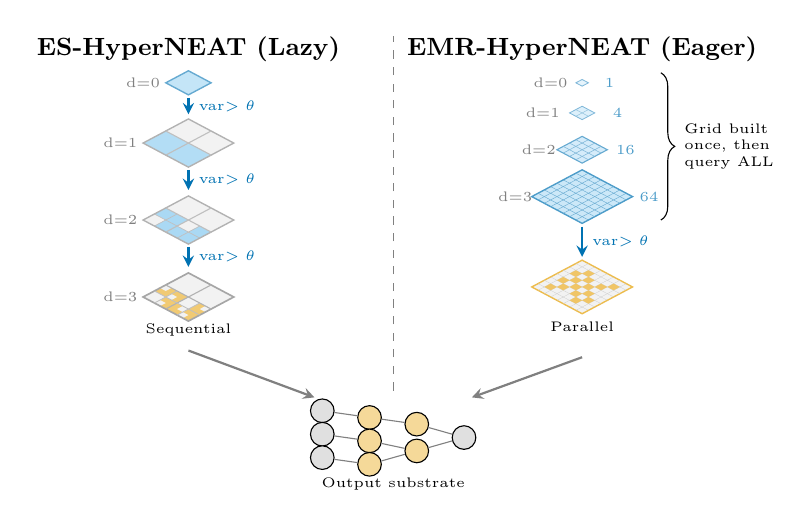
\begin{tikzpicture}[yscale=0.85,
    node distance=0.4cm,
    netnode/.style={circle, draw, fill=oiskyblue!20, minimum size=3mm, inner sep=0pt},
    arrow/.style={->, >=stealth, thick},
    brace/.style={decorate, decoration={brace, amplitude=5pt, mirror}}
]

\pgfmathsetmacro{\ux}{0.08}
\pgfmathsetmacro{\uy}{0.05}

% Left panel - ES-HyperNEAT (Quadtree)
\begin{scope}[shift={(-2.6,0.6)}]
    \node[font=\small\bfseries] at (0,2.0) {ES-HyperNEAT (Lazy)};
    \pgfmathsetmacro{\sx}{1.8}
    \begin{scope}[shift={(0,1.5)}]
        \fill[oiskyblue!35] (0,{2*\uy*\sx}) -- ({2*\ux*\sx},0) -- (0,{-2*\uy*\sx}) -- ({-2*\ux*\sx},0) -- cycle;
        \draw[oiblue!60, line width=0.5pt] (0,{2*\uy*\sx}) -- ({2*\ux*\sx},0) -- (0,{-2*\uy*\sx}) -- ({-2*\ux*\sx},0) -- cycle;
        \node[font=\tiny, gray] at ({-4*\ux*\sx},0) {d=0};
    \end{scope}
    \draw[arrow, oiblue] (0,1.28) -- node[right, font=\tiny] {var$>\theta$} (0,1.03);
    \begin{scope}[shift={(0,0.6)}]
        \fill[oiskyblue!45] (0,0) -- ({-2*\ux*\sx},{2*\uy*\sx}) -- ({-4*\ux*\sx},0) -- ({-2*\ux*\sx},{-2*\uy*\sx}) -- cycle;
        \fill[gray!10] (0,0) -- ({2*\ux*\sx},{2*\uy*\sx}) -- ({4*\ux*\sx},0) -- ({2*\ux*\sx},{-2*\uy*\sx}) -- cycle;
        \fill[gray!10] (0,0) -- ({-2*\ux*\sx},{2*\uy*\sx}) -- (0,{4*\uy*\sx}) -- ({2*\ux*\sx},{2*\uy*\sx}) -- cycle;
        \fill[oiskyblue!45] (0,0) -- ({2*\ux*\sx},{-2*\uy*\sx}) -- (0,{-4*\uy*\sx}) -- ({-2*\ux*\sx},{-2*\uy*\sx}) -- cycle;
        \draw[gray!60, line width=0.5pt] (0,{4*\uy*\sx}) -- ({4*\ux*\sx},0) -- (0,{-4*\uy*\sx}) -- ({-4*\ux*\sx},0) -- cycle;
        \draw[gray!50, line width=0.4pt] ({-2*\ux*\sx},{2*\uy*\sx}) -- ({2*\ux*\sx},{-2*\uy*\sx});
        \draw[gray!50, line width=0.4pt] ({2*\ux*\sx},{2*\uy*\sx}) -- ({-2*\ux*\sx},{-2*\uy*\sx});
        \node[font=\tiny, gray] at ({-6*\ux*\sx},0) {d=1};
    \end{scope}
    \draw[arrow, oiblue] (0,0.2) -- node[right, font=\tiny] {var$>\theta$} (0,-0.1);
    \begin{scope}[shift={(0,-0.55)}]
        \fill[oiskyblue!50] ({-2*\ux*\sx},0) -- ({-3*\ux*\sx},{\uy*\sx}) -- ({-2*\ux*\sx},{2*\uy*\sx}) -- ({-\ux*\sx},{\uy*\sx}) -- cycle;
        \fill[gray!10] ({-2*\ux*\sx},0) -- ({-3*\ux*\sx},{-\uy*\sx}) -- ({-4*\ux*\sx},0) -- ({-3*\ux*\sx},{\uy*\sx}) -- cycle;
        \fill[oiskyblue!50] ({-2*\ux*\sx},0) -- ({-\ux*\sx},{-\uy*\sx}) -- ({-2*\ux*\sx},{-2*\uy*\sx}) -- ({-3*\ux*\sx},{-\uy*\sx}) -- cycle;
        \fill[oiskyblue!50] ({-2*\ux*\sx},0) -- ({-\ux*\sx},{\uy*\sx}) -- (0,0) -- ({-\ux*\sx},{-\uy*\sx}) -- cycle;
        \draw[gray!50, line width=0.25pt] ({-\ux*\sx},{\uy*\sx}) -- ({-3*\ux*\sx},{-\uy*\sx});
        \draw[gray!50, line width=0.25pt] ({-3*\ux*\sx},{\uy*\sx}) -- ({-\ux*\sx},{-\uy*\sx});
        \fill[gray!10] (0,0) -- ({2*\ux*\sx},{2*\uy*\sx}) -- ({4*\ux*\sx},0) -- ({2*\ux*\sx},{-2*\uy*\sx}) -- cycle;
        \fill[gray!10] (0,0) -- ({-2*\ux*\sx},{2*\uy*\sx}) -- (0,{4*\uy*\sx}) -- ({2*\ux*\sx},{2*\uy*\sx}) -- cycle;
        \fill[gray!10] (0,0) -- ({\ux*\sx},{-\uy*\sx}) -- (0,{-2*\uy*\sx}) -- ({-\ux*\sx},{-\uy*\sx}) -- cycle;
        \fill[oiskyblue!50] (0,{-2*\uy*\sx}) -- ({\ux*\sx},{-\uy*\sx}) -- ({2*\ux*\sx},{-2*\uy*\sx}) -- ({\ux*\sx},{-3*\uy*\sx}) -- cycle;
        \fill[oiskyblue!50] (0,{-2*\uy*\sx}) -- ({-\ux*\sx},{-3*\uy*\sx}) -- (0,{-4*\uy*\sx}) -- ({\ux*\sx},{-3*\uy*\sx}) -- cycle;
        \fill[oiskyblue!50] (0,{-2*\uy*\sx}) -- ({-\ux*\sx},{-\uy*\sx}) -- ({-2*\ux*\sx},{-2*\uy*\sx}) -- ({-\ux*\sx},{-3*\uy*\sx}) -- cycle;
        \draw[gray!50, line width=0.25pt] ({\ux*\sx},{-\uy*\sx}) -- ({-\ux*\sx},{-3*\uy*\sx});
        \draw[gray!50, line width=0.25pt] ({-\ux*\sx},{-\uy*\sx}) -- ({\ux*\sx},{-3*\uy*\sx});
        \draw[gray!60, line width=0.5pt] (0,{4*\uy*\sx}) -- ({4*\ux*\sx},0) -- (0,{-4*\uy*\sx}) -- ({-4*\ux*\sx},0) -- cycle;
        \draw[gray!50, line width=0.4pt] ({-2*\ux*\sx},{2*\uy*\sx}) -- ({2*\ux*\sx},{-2*\uy*\sx});
        \draw[gray!50, line width=0.4pt] ({2*\ux*\sx},{2*\uy*\sx}) -- ({-2*\ux*\sx},{-2*\uy*\sx});
        \node[font=\tiny, gray] at ({-6*\ux*\sx},0) {d=2};
    \end{scope}
    \draw[arrow, oiblue] (0,-0.95) -- node[right, font=\tiny] {var$>\theta$} (0,-1.25);
    \begin{scope}[shift={(0,-1.7)}]
        \fill[oiorange!55] (0,0) -- ({-2*\ux*\sx},{2*\uy*\sx}) -- ({-4*\ux*\sx},0) -- ({-2*\ux*\sx},{-2*\uy*\sx}) -- cycle;
        \fill[gray!10] ({-2*\ux*\sx},0) -- ({-3*\ux*\sx},{-\uy*\sx}) -- ({-4*\ux*\sx},0) -- ({-3*\ux*\sx},{\uy*\sx}) -- cycle;
        \fill[gray!10] ({-2*\ux*\sx},{\uy*\sx}) -- ({-2.5*\ux*\sx},{1.5*\uy*\sx}) -- ({-2*\ux*\sx},{2*\uy*\sx}) -- ({-1.5*\ux*\sx},{1.5*\uy*\sx}) -- cycle;
        \fill[gray!10] ({-2*\ux*\sx},{-\uy*\sx}) -- ({-2.5*\ux*\sx},{-0.5*\uy*\sx}) -- ({-3*\ux*\sx},{-\uy*\sx}) -- ({-2.5*\ux*\sx},{-1.5*\uy*\sx}) -- cycle;
        \fill[gray!10] ({-\ux*\sx},0) -- ({-1.5*\ux*\sx},{0.5*\uy*\sx}) -- ({-2*\ux*\sx},0) -- ({-1.5*\ux*\sx},{-0.5*\uy*\sx}) -- cycle;
        \fill[gray!10] (0,0) -- ({2*\ux*\sx},{2*\uy*\sx}) -- ({4*\ux*\sx},0) -- ({2*\ux*\sx},{-2*\uy*\sx}) -- cycle;
        \fill[gray!10] (0,0) -- ({-2*\ux*\sx},{2*\uy*\sx}) -- (0,{4*\uy*\sx}) -- ({2*\ux*\sx},{2*\uy*\sx}) -- cycle;
        \fill[oiorange!55] (0,0) -- ({2*\ux*\sx},{-2*\uy*\sx}) -- (0,{-4*\uy*\sx}) -- ({-2*\ux*\sx},{-2*\uy*\sx}) -- cycle;
        \fill[gray!10] (0,0) -- ({\ux*\sx},{-\uy*\sx}) -- (0,{-2*\uy*\sx}) -- ({-\ux*\sx},{-\uy*\sx}) -- cycle;
        \fill[gray!10] ({\ux*\sx},{-2*\uy*\sx}) -- ({1.5*\ux*\sx},{-1.5*\uy*\sx}) -- ({2*\ux*\sx},{-2*\uy*\sx}) -- ({1.5*\ux*\sx},{-2.5*\uy*\sx}) -- cycle;
        \fill[gray!10] (0,{-3*\uy*\sx}) -- ({-0.5*\ux*\sx},{-2.5*\uy*\sx}) -- ({-\ux*\sx},{-3*\uy*\sx}) -- ({-0.5*\ux*\sx},{-3.5*\uy*\sx}) -- cycle;
        \fill[gray!10] ({-\ux*\sx},{-2*\uy*\sx}) -- ({-0.5*\ux*\sx},{-1.5*\uy*\sx}) -- (0,{-2*\uy*\sx}) -- ({-0.5*\ux*\sx},{-2.5*\uy*\sx}) -- cycle;
        \draw[gray!70, line width=0.6pt] (0,{4*\uy*\sx}) -- ({4*\ux*\sx},0) -- (0,{-4*\uy*\sx}) -- ({-4*\ux*\sx},0) -- cycle;
        \draw[gray!60, line width=0.4pt] ({-2*\ux*\sx},{2*\uy*\sx}) -- ({2*\ux*\sx},{-2*\uy*\sx});
        \draw[gray!60, line width=0.4pt] ({2*\ux*\sx},{2*\uy*\sx}) -- ({-2*\ux*\sx},{-2*\uy*\sx});
        \draw[gray!50, line width=0.3pt] ({-\ux*\sx},{\uy*\sx}) -- ({-3*\ux*\sx},{-\uy*\sx});
        \draw[gray!50, line width=0.3pt] ({-3*\ux*\sx},{\uy*\sx}) -- ({-\ux*\sx},{-\uy*\sx});
        \draw[gray!50, line width=0.3pt] ({\ux*\sx},{-\uy*\sx}) -- ({-\ux*\sx},{-3*\uy*\sx});
        \draw[gray!50, line width=0.3pt] ({-\ux*\sx},{-\uy*\sx}) -- ({\ux*\sx},{-3*\uy*\sx});
        \node[font=\tiny, gray] at ({-6*\ux*\sx},0) {d=3};
    \end{scope}
    \node[font=\tiny, align=center] at (0,-2.2) {Sequential};
\end{scope}

% Right panel - EMR-HyperNEAT (Eager)
\begin{scope}[shift={(2.4,0.6)}]
    \node[font=\small\bfseries] at (0,2.0) {\emrhn{} (Eager)};
    \begin{scope}[shift={(0,1.5)}]
        \fill[oiskyblue!15] (0,\uy) -- (\ux,0) -- (0,-\uy) -- (-\ux,0) -- cycle;
        \draw[oiblue!50, line width=0.3pt] (0,\uy) -- (\ux,0) -- (0,-\uy) -- (-\ux,0) -- cycle;
        \node[font=\tiny, oiblue!70] at (0.35,0) {1};
        \node[font=\tiny, gray] at (-0.4,0) {d=0};
    \end{scope}
    \begin{scope}[shift={(0,1.05)}]
        \fill[oiskyblue!20] (0,{2*\uy}) -- ({2*\ux},0) -- (0,{-2*\uy}) -- ({-2*\ux},0) -- cycle;
        \draw[oiblue!50, line width=0.3pt] (0,{2*\uy}) -- ({2*\ux},0) -- (0,{-2*\uy}) -- ({-2*\ux},0) -- cycle;
        \draw[oiblue!40, line width=0.2pt] ({-\ux},\uy) -- (\ux,-\uy);
        \draw[oiblue!40, line width=0.2pt] ({-\ux},-\uy) -- (\ux,\uy);
        \node[font=\tiny, oiblue!70] at (0.45,0) {4};
        \node[font=\tiny, gray] at (-0.5,0) {d=1};
    \end{scope}
    \begin{scope}[shift={(0,0.5)}]
        \fill[oiskyblue!25] (0,{4*\uy}) -- ({4*\ux},0) -- (0,{-4*\uy}) -- ({-4*\ux},0) -- cycle;
        \draw[oiblue!60, line width=0.4pt] (0,{4*\uy}) -- ({4*\ux},0) -- (0,{-4*\uy}) -- ({-4*\ux},0) -- cycle;
        \foreach \k in {1,2,3} {
            \draw[oiblue!50, line width=0.2pt] ({-4*\ux+\k*\ux},{\k*\uy}) -- ({\k*\ux},{-4*\uy+\k*\uy});
            \draw[oiblue!50, line width=0.2pt] ({-4*\ux+\k*\ux},{-\k*\uy}) -- ({\k*\ux},{4*\uy-\k*\uy});
        }
        \node[font=\tiny, oiblue!70] at (0.55,0) {16};
        \node[font=\tiny, gray] at (-0.55,0) {d=2};
    \end{scope}
    \begin{scope}[shift={(0,-0.2)}]
        \fill[oiskyblue!30] (0,{8*\uy}) -- ({8*\ux},0) -- (0,{-8*\uy}) -- ({-8*\ux},0) -- cycle;
        \draw[oiblue!70, line width=0.5pt] (0,{8*\uy}) -- ({8*\ux},0) -- (0,{-8*\uy}) -- ({-8*\ux},0) -- cycle;
        \foreach \k in {1,...,7} {
            \draw[oiblue!60, line width=0.15pt] ({-8*\ux+\k*\ux},{\k*\uy}) -- ({\k*\ux},{-8*\uy+\k*\uy});
            \draw[oiblue!60, line width=0.15pt] ({-8*\ux+\k*\ux},{-\k*\uy}) -- ({\k*\ux},{8*\uy-\k*\uy});
        }
        \node[font=\tiny, oiblue!70] at (0.85,0) {64};
        \node[font=\tiny, gray] at (-0.85,0) {d=3};
    \end{scope}
    \draw[brace] (1.0,-0.55) -- (1.0,1.65) node[midway, right=5pt, font=\tiny, align=left] {Grid built\\once, then\\query ALL};
    \draw[arrow, oiblue] (0,-0.65) -- node[right, font=\tiny] {var$>\theta$} (0,-1.1);
    \begin{scope}[shift={(0,-1.55)}]
        \fill[gray!10] (0,{8*\uy}) -- ({8*\ux},0) -- (0,{-8*\uy}) -- ({-8*\ux},0) -- cycle;
        \draw[oiorange!70, line width=0.5pt] (0,{8*\uy}) -- ({8*\ux},0) -- (0,{-8*\uy}) -- ({-8*\ux},0) -- cycle;
        \foreach \k in {1,...,7} {
            \draw[gray!40, line width=0.1pt] ({-8*\ux+\k*\ux},{\k*\uy}) -- ({\k*\ux},{-8*\uy+\k*\uy});
            \draw[gray!40, line width=0.1pt] ({-8*\ux+\k*\ux},{-\k*\uy}) -- ({\k*\ux},{8*\uy-\k*\uy});
        }
        \foreach \i/\j in {1/2, 2/1, 2/3, 3/2, 3/4, 4/3, 4/5, 5/4, 5/6, 6/5, 2/5, 5/2, 1/6, 6/1, 3/6} {
            \pgfmathsetmacro{\cx}{(\i-\j)*\ux}
            \pgfmathsetmacro{\cy}{(\i+\j-7)*\uy}
            \fill[oiorange!60] ({\cx},{\cy+\uy}) -- ({\cx+\ux},{\cy}) -- ({\cx},{\cy-\uy}) -- ({\cx-\ux},{\cy}) -- cycle;
        }
    \end{scope}
    \node[font=\tiny, align=center] at (0,-2.15) {Parallel};
\end{scope}

\draw[gray, dashed] (0,-2.5) -- (0,2.8);

% Bottom: Output substrate
\begin{scope}[shift={(0,-2.9)}]
    \draw[arrow, gray] (-2.6,1.0) -- (-1.0,0.3);
    \draw[arrow, gray] (2.4,0.9) -- (1.0,0.3);
    \node[netnode, fill=oigray!30] (i1) at (-0.9,0.1) {};
    \node[netnode, fill=oigray!30] (i2) at (-0.9,-0.25) {};
    \node[netnode, fill=oigray!30] (i3) at (-0.9,-0.6) {};
    \node[netnode, fill=oiorange!40] (h1a) at (-0.3,0.0) {};
    \node[netnode, fill=oiorange!40] (h1b) at (-0.3,-0.35) {};
    \node[netnode, fill=oiorange!40] (h1c) at (-0.3,-0.7) {};
    \node[netnode, fill=oiorange!40] (h2a) at (0.3,-0.1) {};
    \node[netnode, fill=oiorange!40] (h2b) at (0.3,-0.5) {};
    \node[netnode, fill=oigray!30] (o1) at (0.9,-0.3) {};
    \draw[gray, line width=0.4pt] (i1) -- (h1a); \draw[gray, line width=0.4pt] (i2) -- (h1b);
    \draw[gray, line width=0.4pt] (i3) -- (h1c); \draw[gray, line width=0.4pt] (h1a) -- (h2a);
    \draw[gray, line width=0.4pt] (h1b) -- (h2b); \draw[gray, line width=0.4pt] (h1c) -- (h2b);
    \draw[gray, line width=0.4pt] (h2a) -- (o1); \draw[gray, line width=0.4pt] (h2b) -- (o1);
    \node[font=\tiny, align=center] at (0,-1.0) {Output substrate};
\end{scope}
\end{tikzpicture}%
\end{document}
